\documentclass[aspectratio=169,12pt]{beamer}
\usepackage{beamerthemeTalentSprint}
\usepackage{fancybox}
\usepackage{graphics}
\usepackage{blkarray}
\usepackage{ragged2e}
\usepackage{graphicx}
\usepackage{rotating}
\usepackage{caption}
\usepackage{amsmath}
\usepackage{subcaption}
\usepackage{amsfonts}
\usepackage{xcolor}
\usepackage{multicol}
\usepackage{tcolorbox}
\usepackage{setspace}
\usepackage{rotating}
\setlength{\columnsep}{1cm}
\definecolor{swe}{rgb}{0.19, 0.73, 0.56}



\begin{document}

{\1
\begin{frame}
	\title{Web Scraping}​
\titlepage
\end{frame}
}



\begin{frame}[t]{Access data from Websites}
\begin{itemize}
\itemsep2em 
\item Web scrapingis a technique for gathering data or information from websites.
\item We can extract any data which we can see while browsing the web. 
\item We can save the data to a local file in your computer or to a 
database in table (spreadsheet) format using Pandas library.
\end{itemize}
\end{frame}

\begin{frame}{Web Scraping}
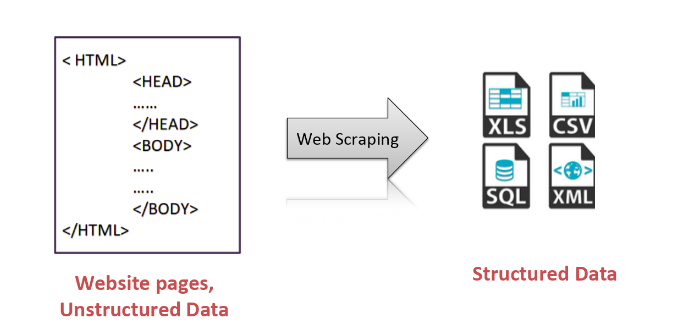
\includegraphics[width=0.9\textwidth,height=0.7\textheight]{Images/AIML_WS_IMG1.png}
\end{frame}

\begin{frame}{Web Scraping Workflow​}
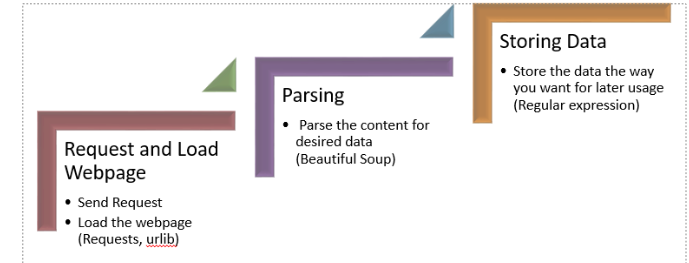
\includegraphics[width=0.9\textwidth,height=0.7\textheight]{Images/AIML_WS_IMG4.png}
\end{frame}

\begin{frame}{Performing HTTP Request in Python}
\begin{columns}
\column{0.5\textwidth}

\begin{itemize}
\itemsep1em
 
\item Import requests module
\item Download the html page from the specific resource 
\item Get the content from requested html page
\end{itemize}
\column{0.5\textwidth}
	\begin{flushright}
		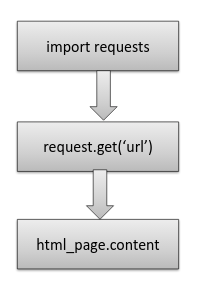
\includegraphics[width=6cm,  height=5.5cm]{Images/AIML_WS_IMG2.png}
	\end{flushright}

\end{columns}
\end{frame}


\begin{frame}[t]{Parsing the data}
\begin{itemize}
\itemsep2em 
\item HTML is nested, cannot extract data simply through string processing.
\item Need parser to create a tree structure of the HTML data. 
\item  Use \textbf{Beautiful} Soup for parsing the HTML data.
\item We can extract any specific data like author name, title, tables and description.
\end{itemize}
\end{frame}


\begin{frame}{Beautiful Soup​}
\begin{columns}
\column{0.5\textwidth}

\begin{itemize}
\itemsep1em 
\item Import BeautifulSoup
\item Parse the html page
\item Extract the text without any HTML Tags
\item  Store the data in a required format
\end{itemize}
\column{0.5\textwidth}
	\begin{flushright}
		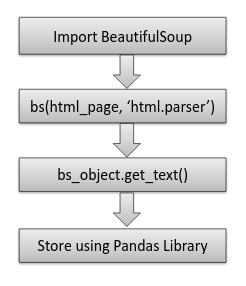
\includegraphics[width=6cm,  height=5.5cm]{Images/AIML_WS_IMG3.png}
	\end{flushright}

\end{columns}
\end{frame}

\begin{frame}{Experiments : }
\begin{itemize}
\item \href{https://drive.google.com/file/d/1MY9I-HIv906SL2TKUZ_kNDvxhlTH1Mzu/view?usp=sharing}{Demo\_Web\_Scraping} 
	\begin{itemize}
		\item Objective :  Extract data from web page using Beautiful Soup
	\end{itemize}

\end{itemize}
\end{frame}

{\1
\begin{frame}[plain,noframenumbering]
\title{Natural Language Toolkit}
\subtitle{(NLTK)}
  \titlepage
\end{frame}
}




\begin{frame}[t]{NLTK Package}
\begin{itemize}
\itemsep0em 
\item One of the most powerful NLP libraries which contains packages to make machines understand human language.
\item Tokenization helps in interpreting the meaning of the text by splitting string, text into a list of tokens. 
\item Punkt module for splitting the paragraphs into sentences, sentences into words. 
\item Wordnet is a tool integrated into NLTK that contain listings of word relations.
\item ImageNet is a largescale ontology of images built upon the backbone of the WordNet structure. ImageNet constitutes \_∼ 10\_% of the WordNet synsets
\end{itemize}
\end{frame}

\begin{frame}[t]{NLTK Basic Functionalities}
\begin{itemize}
\itemsep1em 
\item Sentence Tokenization
\item Word Tokenization
\item Parts of Speech (POS) tagging
\item Stemming and Lemmatization
\item Stop words removal
\end{itemize}
\end{frame}

\begin{frame}[t]{Text Analytics}
\begin{itemize}
\itemsep2em 
\item \textbf{Sentence} Tokenization means breaking down a paragraph into sentences.
\item \textbf{Word Tokenization} means breaking down a paragraph into words.
\item \textbf{Parts of Speech (POS) tagging} looks for relationship within the sentence and assigns label for each word with
its appropriate parts of speech. 
\end{itemize}
\end{frame}

\begin{frame}[t]{Pre-Processing Text}
\begin{itemize}
\itemsep1em 
\item \textbf{Stemming} reduces the word to the root word\\
\alert - was - wa; studies - studi; studying - study
\item \textbf{Lemmatization} is similar to stemming but is related to grammatical context\\
\alert - was - be; studies - study; studying - study
\item \textbf{Stop words}  Noise in the text. Text may contain stop words such as its appropriate parts of speech. \\
\alert - is, am, at, of, are this, a, the, an.
\item Remove these stop words from the list of words
\end{itemize}
\end{frame}


\begin{frame}{Experiments : }
\begin{itemize}
\item \href{https://drive.google.com/file/d/1Z8ogpw23P4GarSHCdTJQ_MeHVQTJ2xNg/view?usp=sharing}{Demo\_NLTK} 
	\begin{itemize}
		\item Objective : Text pre-processing using NLTK
	\end{itemize}

\end{itemize}
\end{frame}

\begin{frame}
\begin{center}
\centering 
\textbf{\textcolor{orange}{\Huge \vspace{8pt} Thanks!!\\}}
\textcolor{white}{\\}
\centering
\textbf{\textcolor{black}{\Huge \textcolor{white}{-}Questions?}}
\end{center}
\end{frame}

\end{document}





